%%%%%%%%%%%%%%%%%%%%%%%%%%%%%%%%%%%%%%%%%
% a0poster Portrait Poster
% LaTeX Template
% Version 1.0 (22/06/13)
%
% The a0poster class was created by:
% Gerlinde Kettl and Matthias Weiser (tex@kettl.de)
% 
% This template has been downloaded from:
% http://www.LaTeXTemplates.com
%
% License:
% CC BY-NC-SA 3.0 (http://creativecommons.org/licenses/by-nc-sa/3.0/)
%
%%%%%%%%%%%%%%%%%%%%%%%%%%%%%%%%%%%%%%%%%

%----------------------------------------------------------------------------------------
%	PACKAGES AND OTHER DOCUMENT CONFIGURATIONS
%----------------------------------------------------------------------------------------

\documentclass[a0,portrait]{a0poster}

\usepackage{multicol} % This is so we can have multiple columns of text side-by-side
\columnsep=100pt % This is the amount of white space between the columns in the poster
\columnseprule=3pt % This is the thickness of the black line between the columns in the poster

\usepackage[svgnames]{xcolor} % Specify colors by their 'svgnames', for a full list of all colors available see here: http://www.latextemplates.com/svgnames-colors

%\usepackage{times} % Use the times font
\usepackage{palatino} % Uncomment to use the Palatino font

\usepackage{graphicx} % Required for including images
\usepackage{booktabs} % Top and bottom rules for table
\usepackage[font=Large,labelfont=bf]{caption} % Required for specifying captions to tables and figures
\usepackage{amsfonts, amsmath, amsthm, amssymb} % For math fonts, symbols and environments
\usepackage{wrapfig} % Allows wrapping text around tables and figures
\usepackage{wrapfig} % Allows wrapping text around tables and figures
\usepackage{caption}
\usepackage{algorithm}
%\let\algorithmic\relax
%\usepackage{algorithmic}
\usepackage{algpseudocode}
\usepackage{subfigure}
\usepackage{array}
\begin{document}

%----------------------------------------------------------------------------------------
%	POSTER HEADER 
%----------------------------------------------------------------------------------------

% The header is divided into two boxes:
% The first is 75% wide and houses the title, subtitle, names, university/organization and contact information
% The second is 25% wide and houses a logo for your university/organization or a photo of you
% The widths of these boxes can be easily edited to accommodate your content as you see fit

\begin{minipage}[b]{0.75\linewidth}
\veryHuge \color{NavyBlue} \textbf{Smart House (Remote light control)} \color{Black}\\ % Title

\huge \textbf{Group 7: Sahand Sabour, Jiamin Wang, Tingyu Lin, Mengqing Zhao, and Kai-Yu Lu}\\[0.5cm] % Author(s)
\huge Department of Electrical and Electronic Engineering\\[0.4cm] % University/organization
\huge Supervisor: Dr. T.O. Ting\\
\end{minipage}
%
\begin{minipage}[b]{0.25\linewidth}
\includegraphics[scale=2.8]{img/logo}\\
\end{minipage}

\vspace{0.5cm} % A bit of extra whitespace between the header and poster content

%----------------------------------------------------------------------------------------

\begin{multicols}{2} % This is how many columns your poster will be broken into, a portrait poster is generally split into 2 columns

%----------------------------------------------------------------------------------------
%	ABSTRACT
%----------------------------------------------------------------------------------------

\color{Navy} % Navy color for the abstract

\section*{Abstract}
\Large
As Internet of Things (IoT) has revolutionized the modern life, this project aims to build a simple prototype of the Smart House, which can be controlled and monitored by a WeChat mini program. The model implements remote control of the lights as well as monitor of the front door's status through Wi-Fi. The transmission time of the model is around 5 seconds while the success rate is approximately 100\%. In terms of improvements, we plan to implement 5G technology to enhance the model's network and add security measures to address its current privacy issues.

%----------------------------------------------------------------------------------------
%	INTRODUCTION
%----------------------------------------------------------------------------------------

\color{SaddleBrown} % SaddleBrown color for the introduction
\section*{Introduction}
\Large
In the modern world, the need for connectivity rises and the remote control of electronic devices has become one of the main objectives of great companies \cite{shang2012internet}. It has caused the rise of Internet of Things (IoT) and the concept of Smart house \cite{yang2018iot}. Smart House allows remote access to monitor and manage household appliances, which would be more time-efficient and convenient for users. Our group aims to build a small model of the Smart House which can be controlled by a WeChat mini-program.


\color{DarkSlateGray} % Set the color back to DarkSlateGray for the rest of the content

%----------------------------------------------------------------------------------------
%	MATERIALS AND METHODS
%----------------------------------------------------------------------------------------
\setcounter{secnumdepth}{2}
\section*{Methodology}
\Large
In our project, there are four parts regarding the methodology. Firstly, we built a small-scale house model to simulate a real life household. (See Fig. \ref{House model}). Accordingly, two PHP files were created to process clients' requests (See Fig. \ref{Server design}). To avoid the complicated connection between the ESP module and the basic UNO board, we applied an improved board, which is known as NodeMCU, instead. The complete hardware circuit is shown in Fig. \ref{Arduino design}. Regarding the software part of the Arduino design , we merely used two libraries: \\
\textbf{ESP8266WiFi.h} - connect to a given Wi-Fi network \\
\textbf{ESP8266HTTPClient.h} - send HTTP requests\vspace{0.5em}
%\noindent There are two types of requests that needed to be sent.\\
%\vspace{-1.2em}
%\begin{itemize}
%	\item GET request - obtain the status of each LED	
%	\item SET request - update the current status of the door
%\end{itemize}

\noindent Consequently, our team designed a WeChat mini-program which can be run on various operating system (See Fig. \ref{UI}). This mini app allows the user to turn the lights on/off by using the corresponding buttons. Moreover, the status of devices would update automatically.

\begin{center}
	\begin{figure}[H]
		\begin{tabular}{cc}
			
			\subfigure[House model]{
				%\begin{minipage}[t]{0.5\textwidth}
				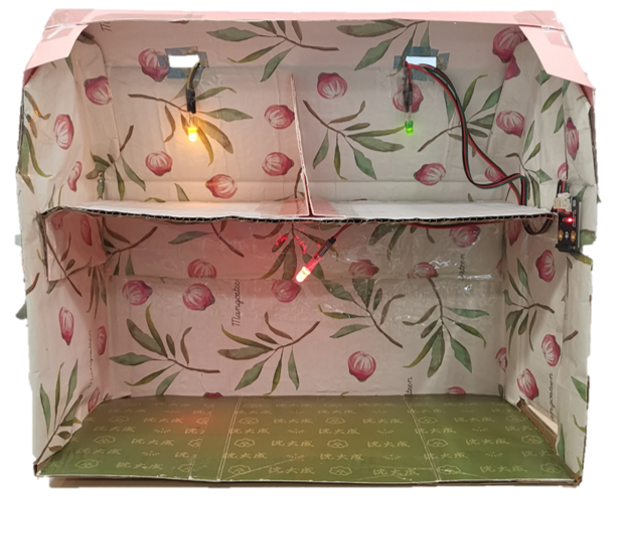
\includegraphics[width=17cm,height=9cm]{img/house.png}
				\label{House model}
			}					
			
			\subfigure[Two PHP files]{
				%\begin{minipage}[t]{0.5\textwidth}
				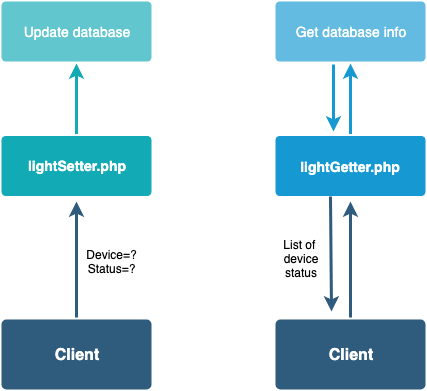
\includegraphics[width=17cm,height=9cm]{img/server.png}
				\label{Server design}
			}
		\end{tabular}
	
		\begin{tabular}{cc}
			
			\subfigure[The whole circuit]{
				%\begin{minipage}[t]{0.5\textwidth}
				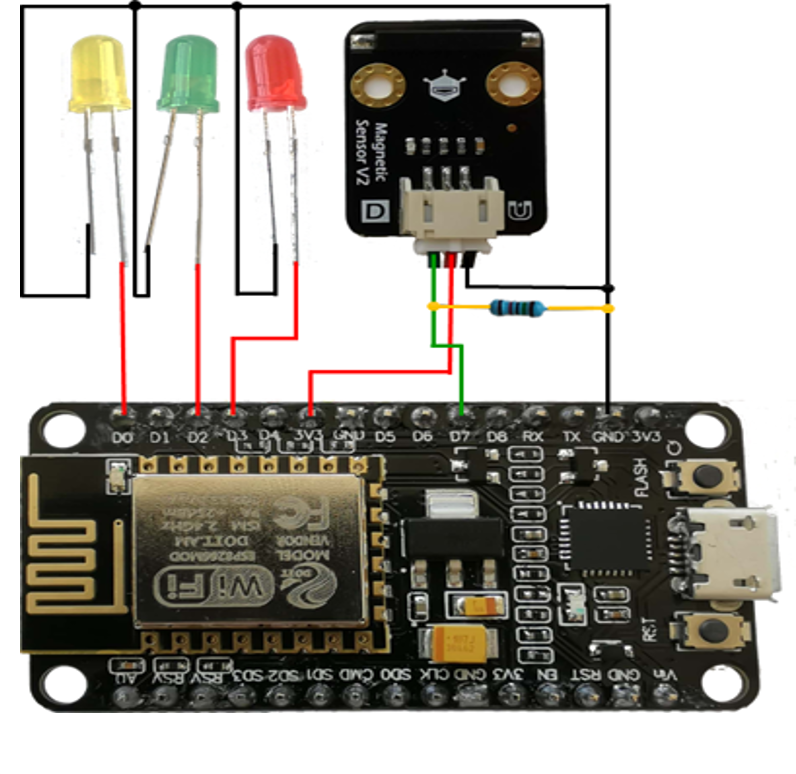
\includegraphics[width=17cm,height=9cm]{img/circuit.png}
				\label{Arduino design}
			}

			\subfigure[User interface of WeChat mini-program]{
				%\begin{minipage}[t]{0.5\textwidth}
				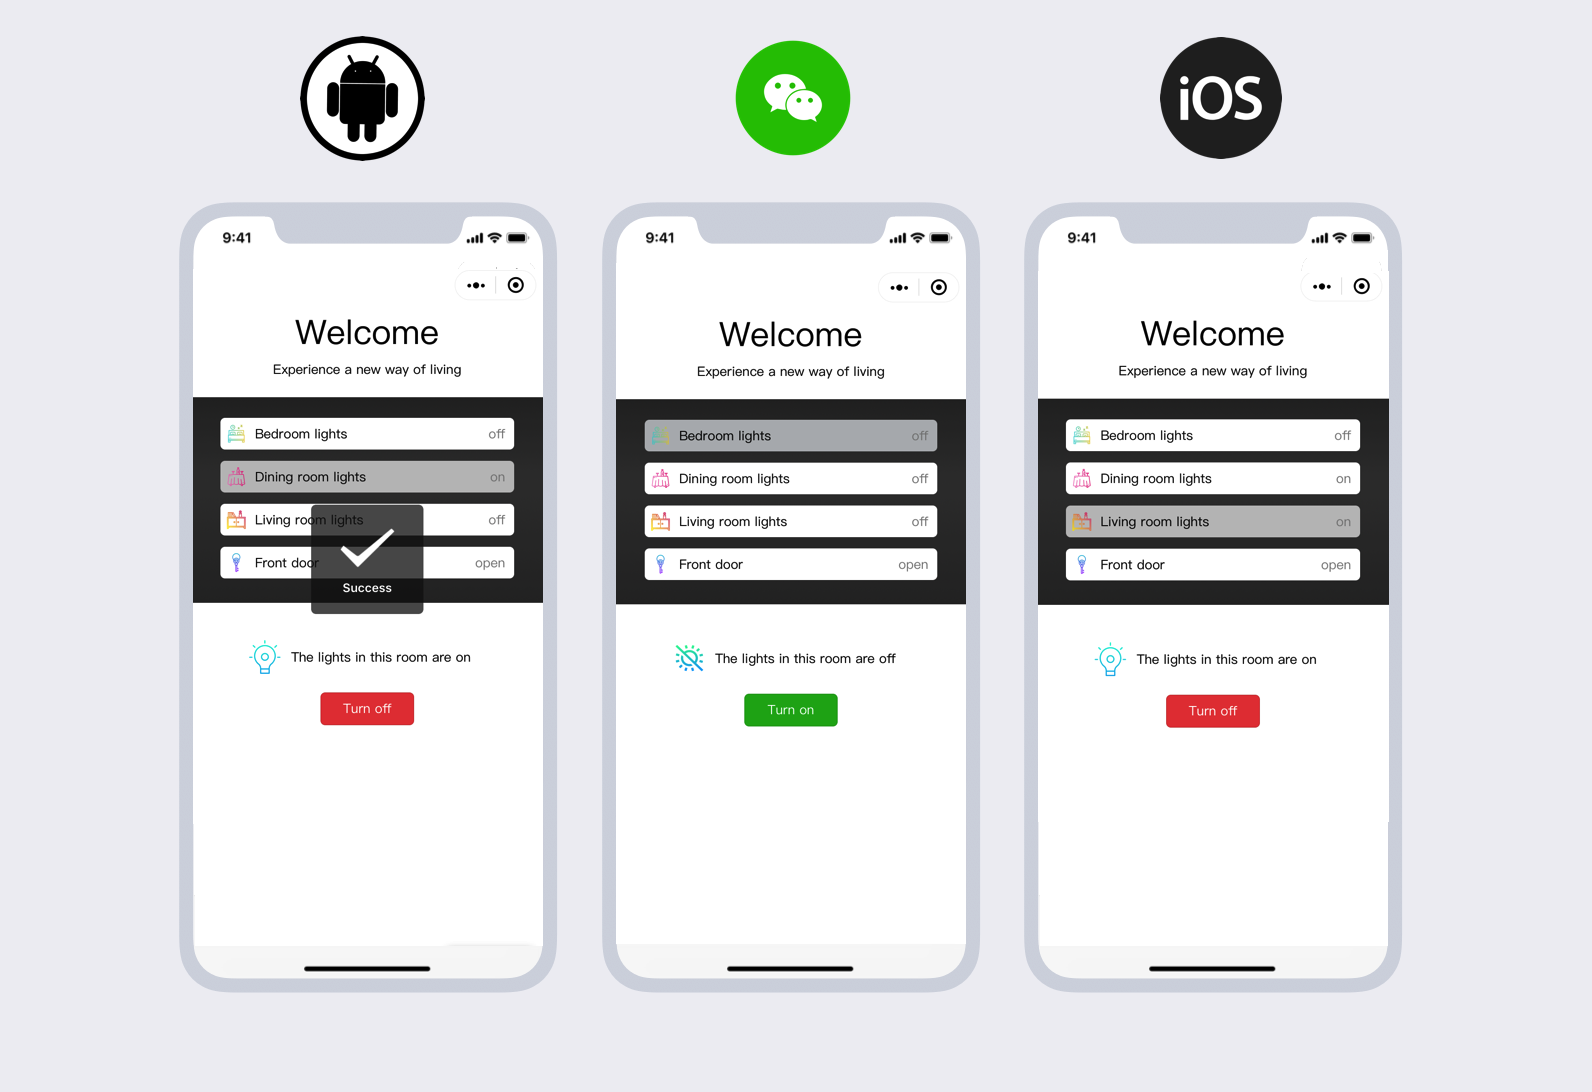
\includegraphics[width=17cm,height=9cm]{img/UI.png}
				\label{UI}
			}
		
		\end{tabular}			
	\end{figure}
	\captionof{figure}{\color{Navy} The four parts of the methodology}
	\label{methodology}
\end{center}
%----------------------------------------------------------------------------------------
%	RESULTS 
%----------------------------------------------------------------------------------------
\color{Navy}
\vspace{-2em}
\section*{Results}
\Large
\setcounter{subsection}{0}
\renewcommand\thesubsection{\Roman{subsection}}
\subsection{\Large Testing reusult}
\vspace{-0.5em}
The model was connected to power bank with 5.1V / 2.1A and a personal hotspot. After establishing the required power and connection for this prototype, we randomly tested and measured the transmission time of the LEDs and the door ten times (See Fig. \ref{Testing}).
\begin{center}
	\begin{figure}[H]
		\begin{tabular}{cc}
			\subfigure[Three LEDs transmission time]{
				%\begin{minipage}[t]{0.5\textwidth}
				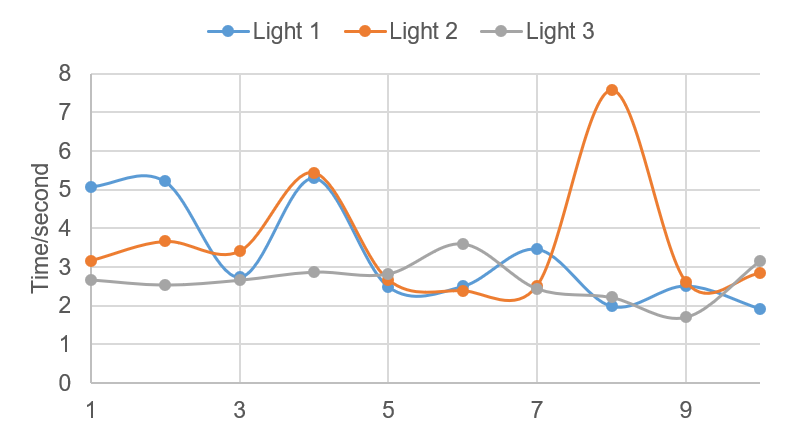
\includegraphics[width=17cm,height=10cm]{img/light_result.png}
				\label{LEDs}
			}					
			
			\subfigure[The door transmission time]{
				%\begin{minipage}[t]{0.5\textwidth}
				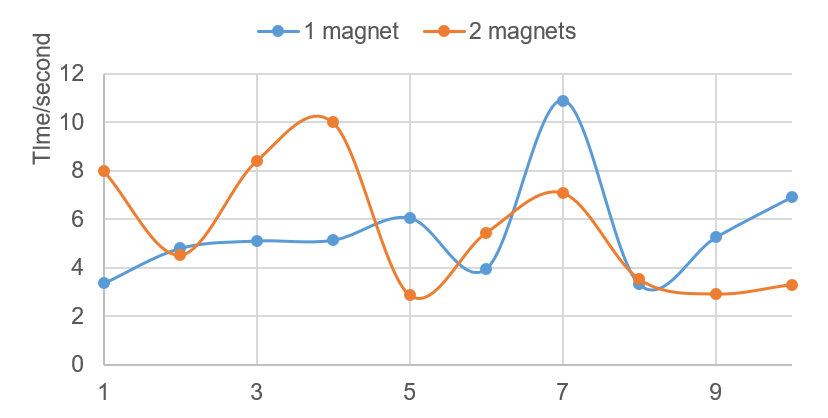
\includegraphics[width=17cm,height=10cm]{img/door_result.png}
				\label{Door}
			}
		\end{tabular}		
	\end{figure}
	\captionof{figure}{\color{Navy} Measurements of transmission time}
	\label{Testing}
\end{center}
\vspace{-1.2em}
\noindent The average transmission time is computed in Table \ref{table_results}.
\vspace{-0.5em}
\color{Black}
\begin{center}
\captionof{table}{\color{Navy} Testing results of transmission time} \label{table_results}
{
	\begin{tabular}{p{8cm}<{\centering}  p{8cm}<{\centering}  p{8cm}<{\centering} }
	\toprule
	 & \textbf{Lights} & \textbf{Door} \\
	\hline
	$\bar{t}(s)$ &  3 & 5.5 \\
	Accuracy &  \multicolumn{2}{c}{100 \%} \\
	\bottomrule
	\end{tabular}
}
\end{center}
\vspace{-1em}
\color{Navy}
\subsection{\Large Discussion}
\vspace{-0.5em}
Due to the I/O pin being highly sensitive to electrical noise, random fluctuations occur in I/O between the connection pins. This is phenomena is known as the floating pin. In order to resolve this issue, we inserted a pull-up 15k$\Omega$ resistor between I/O and GND pins (See Fig.\ref{Arduino design}). 

%----------------------------------------------------------------------------------------
%	CONCLUSIONS
%----------------------------------------------------------------------------------------

\color{SaddleBrown} % SaddleBrown color for the conclusions to make them stand out

\section*{Future works and Conclusions}
\Large
In order to reduce the transmission delay, we plan to implement 5G to improve this project. Additionally, we would deploy the server in a local city due to the same reason. Moreover, our team plans to add owner authorization, user verification, and data encryption to the WeChat mini-program by applying Hash Codes. This would address the privacy and security issues that our current prototype has.
In conclusion, our team was able to successfully build a properly functioning prototype of the Smart House, where the user can control and monitor the lights in the house as well as its front door.

\color{DarkSlateGray} % Set the color back to DarkSlateGray for the rest of the content


 %----------------------------------------------------------------------------------------
%	REFERENCES
%----------------------------------------------------------------------------------------
\nocite{*} % Print all references regardless of whether they were cited in the poster or not
\bibliographystyle{IEEEtran} % Plain referencing style
\bibliography{ref} % Use the example bibliography file sample.bib

%----------------------------------------------------------------------------------------
%	ACKNOWLEDGEMENTS
%----------------------------------------------------------------------------------------

\section*{Acknowledgement}
\large

Special thanks to Dr. T.O. Ting for his supervision and critical criticism that made this project significantly more functional and meaningful.

%----------------------------------------------------------------------------------------

\end{multicols}
\end{document}